% used labels:
% Figures (fig):
% 	dashboard
%	openstack_services_arch
% 	os_arch
% 	ph115_t40
% 	vm115_large_wobs
% 	vm115_physical_wobs
% 	vm115_large_wbs
% 	vm115_physical_wbs
% 	vm116_large_wbs
% 	vm116_physical_wbs
% 	vm_large_iso
% 	
% 	
% 	
% 	
% Tables (table):
%	flavors_list
%	flavors_list_2
%	hdparm_res_PM
%	hdparm_res_VM
%	oltpbench_list
% 	openstack_services_list
% 	storage_list
% 	tpcc_trans_type_list
% 	tab_oltpb_scalefactor
% 	
% Listings (lst):
% 	lst_cmd_oltpsh
% 	lst_cmd_oltpb_cloning
% 	lst_cmd_oltpbenchmark
% 	lst_cmd_others_install
% 	lst_oltp_script
% 	lst_oltp_config
% 	lst_cmd_mount_movedb
% 	lst_apparmor
% 	
% Sections:
% 	section_setup
% 	
% 	
% Equation (eq):
% 	eq_iqr






% use "amsart" instead of "article" for AMSLaTeX format
\documentclass[a4paper, 12pt, oneside, titlepage]{scrbook}
% See geometry.pdf to learn the layout options. There are lots.
\usepackage[margin=1.0in]{geometry}
\geometry{letterpaper}

% Activate for for rotated page geometry
%\geometry{landscape}

% Activate to begin paragraphs with an empty line rather than an indent
%\usepackage[parfill]{parskip}

% Use pdf, png, jpg, or eps§ with pdflatex; use eps in DVI mode
% TeX will automatically convert eps --> pdf in pdflatex
\usepackage{graphicx}
\usepackage{fancyhdr}
\usepackage{amssymb}

\usepackage[utf8]{inputenc}
\usepackage[T1]{fontenc}

\usepackage{setspace}
\usepackage{array}
\usepackage{csquotes}
\usepackage{hyperref}
\usepackage{textcomp}
\usepackage{multirow}
\usepackage{url}

\usepackage[usenames,svgnames]{xcolor}
\usepackage{listings}
\lstset{
  %basicstyle=\ttfamily,
  basicstyle=\footnotesize\ttfamily,
  showstringspaces=false,
  commentstyle=\color{gray},
  keywordstyle=\color{blue}
}

\pagestyle{fancyplain}
\fancyhf{}
\rhead{\fancyplain{} \rightmark}
\lfoot{}
\cfoot{\fancyplain{} \thepage}
\rfoot{}
\fancypagestyle{plain}

\newcommand{\rp}[1]{\textcolor{Magenta}{RP: #1}}



\begin{document}


%%--------------- TITLE
\begin{titlepage} 
	\begin{center}
		
		
\includegraphics[scale=0.4]{figures/UNF_Signet_100pr_pos.jpg}\\
		
		\vspace{0.5cm}
		
		University of Fribourg, Switzerland\\
		Faculty of Science\\
		Department of Informatics\\
		eXascale Infolab\\

		\vspace{1.5cm}

		\begin{huge}
			%Sans serif
			{\sf \textbf{Benchmarking Open Source}}\\
			\vspace{0.3cm}
			{\sf \textbf{Cloud Computing Solutions}}
		\end{huge}
		
				
		\vspace{1.5cm}

		Bachelor Work\\

		\vspace{1cm}
		
		Nadia \textsc{Aebischer}\\
		Rte des Pervenches 3\\
		1700 Fribourg\\
		Suisse\\
		Immatriculation number: 10-211-886\\
		E-mail: nadia.aebischer@unifr.ch\\

		\vspace{1cm}

		Instructor:\\
		Prof. Dr. Philippe \textsc{Cudré-Mauroux}\\

		\vspace{0.5cm}
		
		Person in charge:\\
		Roman \textsc{Prokofyev}\\

		\vspace{1cm}

		\today
				
	\end{center}
\end{titlepage}

\tableofcontents
\listoffigures
\listoftables
\doublespacing



%%--------------- abstract
\chapter*{Abstract}
% TODO: complete abstract
Enter your abstract here

{\bf Keywords:} OpenStack, Open cloud, IaaS, Virtualization, Benchmark, TPC-C.


%%--------------- section
%% Introduction


\chapter{Introduction}
Since several years, \textit{Cloud Computing} gained in popularity, mostly because it allows companies and individuals to store or analyze large amount of data with reduced costs. 
In the domain of \textit{Cloud Computing}, most individuals are only using softwares or services made available by third parties. 
As examples, we can mention Gmail from Google, which lets you send and receive e-mails, or Drive from Google for storing and sharing your documents. 
The webmail services have been around for several years and are using the \textit{Cloud Computing}. 
Indeed, the users don't need to care about the installation or the update of the server. 
All they need to do is to use the available service. Continuing our webmail example, the users don't need to know where and how their e-mails are stored, as long as they are stored somewhere accessible remotely. This is all the interest about \textit{Cloud Computing} for the end users.

Concerning the companies, they are more and more that want to store and analyze their data to better understand their clients. 
The amount of these data can be counted in terabytes or even petabytes. 
To deal with such a enormous amount of data powerful systems are needed. 
However, all companies, especially the startups, have not the means to invest in new systems, because it will cost too much (machines, installation, maintenance, etc). 
Moreover, if the amount of data or computations a company deals with growth too fast, it will take too long to install new systems, and thus it will take longer to analyze all the data. 
\textit{Cloud Computing} helps by quickly adding more storage, more RAM or even more CPUs depending on your needs. 
The basic principal of \textit{Cloud Computing} is to provide hardware resources easily and rapidly over the Internet.

From these few examples, we can see how convenient \textit{Cloud Computing} can be, either for companies or individuals. 
This is why thie market has been growing more and more these past years. 
Among the major players in the cloud, we can mention Amazon and Google. 
Amazon is the most known for its cloud services AWS (Amazon Web Services), which let the user create a server (i.e. a virtual machine) in a few mouse clicks and begin to develop on it. 
This can be very useful for companies, for example, if tomorrow, your company needs a new server to deal with a growing demand, no problem, a new (virtual) server can be created in a blink of an eye with Amazon. 
It's a service on demand and where the clients only need to pay what they consume (i.e. computing power). 
Moreover, the company using this service doesn't need to care about the machines maintenance, which is done by the one proposing the service.



\section{Motivation and method}
\textit{Cloud Computing} is very interesting because one can easily add computing power to deal with a growing project. 
The goal of this bachelor work was to experience with open source cloud computing solutions. 
OpenStack, one of the biggest open source project (and free) out there, was chosen for this bachelor work. 
It offers the possibility to create its own cloud infrastructure, which can then be managed through a provided web interface.

At first, OpenStack will be installed and condifured on three chosen physical machines. 
Once everything is working correctly, OpenStack will be benchmarked with the help of OLTP-Bench, another open source project. 
OpenStack will be benchmarked with different configurations and the same benchmark will run on the physical machines as a point of comparison.


% \section{Method}



%%--------------- section
%!TEX root = ../main.tex
%% Chapter 1 - Cloud Computing


\chapter{Cloud Computing}
During the last decade, \textit{Cloud Computing} technology got a lot of traction, but many people do not know what this technology stands for exactly. 
In fact, we all use cloud computing since several years without actually knowing it. One prominent example is webmail, a service which gives a possibility to send and receive e-mails.
More formally, \textit{Cloud Computing} offers users a possibility to do something (i.e. writing a text document) on the web without the need to have any software installed locally, everything is being done on a remote server. 
This is exactly what is being offered to the users by webmail services.

When talking about the \textit{cloud}, one must make the difference between private, hybrid and public clouds. 
A private cloud allows to have the advantages of the cloud, but it is restrained to the organization, meaning that it is not exposed to the Internet and that all the hardware resources (i.e. servers) reside inside the organization. 
Thus the services are accessible only when the employees are connected to the internal network of the organization. 
On the other hand, a public cloud is exposed to the Internet, meaning that we can access it from everywhere as long as we have an Internet connection. 
A good example is \textit{Dropbox}\footnote{\url{https://dropbox.com}} service, which offers the possibility to store data in the cloud. 
In the middle, there is the hybrid cloud, which is a mix of the previous two types of clouds.

In addition to the three types presented earlier, there exist several cloud models.
The three most important ones are IaaS, PaaS and SaaS \rp{give non-acronym versions first, probably make a list.}, which will be presented in the next sections. 
These proposed models are not always free, or in most cases they are free with a limited access to resources \rp{You're mixing a bit companies that provide services and models themselves, cloud model have nothing to do with pricing, they are just abstractions, I suggest to remove this and the next sentence.}. 
For intensive usage, the client (in general the company) must pay a monthly fee to the one provisioning the service.





%%--------------- subsection
\section{SaaS}
\textit{Software as a Service} (SaaS) model represents a remotely accessible software that is provided to the users. 
This type of software is also known as a hosted service. 
The software is accessible through Internet and the Web, so the user does not need to install anything on its own machine. 
Typical examples of such software are in businesses domain, such as Enterprise Resource Planning (ERP) and Customer Relationship Management (CRM) solutions. 
A more common piece of software is the webmail (e.g. Gmail), which lets users read and receive their e-mails without the need to install any mail client. 
Webmail services mentioned before also fall into this category. 
Another interesting example is the \textit{Google Drive}\footnote{\url{https://drive.google.com}} service, which lets users create and share documents, spreadsheets and presentation slides straight from a web browser. 
The user does not need to install any additional software to access it (except the web browser). 
As can be seen, this software is clearly intended for end users, who do not have to worry about security updates and all this stuff \rp{this is not scientific ;), try to rewrite somehow}, as this is entirely taken care by the one providing the applications.



%%--------------- subsection
\section{PaaS}
 \textit{Platform as a Service} (PaaS) model is intended for developing and deploying applications on an existing infrastructure.
Unlike SaaS, this model is designed for application developers so they do not need to install, configure or maintain any infrastructure (servers, network, etc.) as this is taken care by a PaaS provider. 
This way, PaaS fosters the work of developers by freeing them from system administration work. 
OpenShift, Heroku and Google App Engine are examples of PaaS providers \rp{create footnotes for every service mentioned as I did before}.
All these companies provide ready-to-use environments for developing applications.
The developers just need to choose the programming language in which they want to code and eventually also the framework and the database system, and everything is ready to start the development.



%%--------------- subsection
\section{IaaS}
IaaS stands for \textit{Infrastructure as a Service} and means that infrastructure resources, like CPU, memory, storage, servers, are provided to the client on demand. A better definition of an infrastructure could be:
\begin{quotation}
\textit{
IT infrastructure refers to the composite hardware, software, network resources and services required for the existence, operation and management of an enterprise IT environment. It allows an organization to deliver IT solutions and services to its employees, partners and/or customers and is usually internal to an organization and deployed within owned facilities.
}\cite{cjanssen14}
\end{quotation}

IaaS is not intended to final users, but to network architects, whose work is to 
\textit{design and implement data communications networks, and computer and information networks including limited area networks, wide area networks, intranets, and extranets.}\footnote{\url{https://www.recruiter.com/salaries/computer-network-architects-salary/}, 14.01.2015}

Thanks to IaaS, companies don't have to spend money to buy new hardware to run their business, they can simply rent these hardware with the computing power they want, and it will be easy to add more computing power later if they need to and vice-versa. 
Moreover, they don't need to worry about the hardware itself as it's not owned by the company (in case of a public cloud). 
One of the most famous company proposing these services is Amazon. 
Their service Amazon Elastic Compute Cloud (Amazon EC2). 
For this bachelor work, we'll be using similar services offered by OpenStack, which will be presented in more details later.

Taking a step further, recently another type of model has grown: MaaS, standing for \textit{Metal as a Service} proposed by Canonical. 

\begin{quotation}
\textit{A system that makes it quick and easy to set up the physical hardware on which to deploy complex scalable services, like Ubuntu’s OpenStack cloud infrastructure.}\footnote{\url{http://www.ubuntu.com/cloud/tools/maas}, 14.01.2015}
\end{quotation}

Contrary to IaaS, the goal of MaaS is to provide real servers on demand with the speed of a cloud instance. Then with the help of Juju it is easier to deploy a IaaS like OpenStack on the hardware.









%%--------------- section
%!TEX root = ../main.tex
%% Chapter 2 - Openstack


\chapter{OpenStack}

This section gives a detailed description of the \textit{OpenStack} technology in order to better understand how it works.


%%--------------- section
\section{Definition}
\textit{OpenStack} is an open source project licensed under the \textit{Apache License 2.0} and consists of several projects (or services), which allow creating cloud infrastructures.
In other words it is \textit{a cloud operating system that controls large pools of compute, storage, and networking resources throughout a data center, all managed through a dashboard that gives administrators control while empowering their users to provision resources through a web interface.
}\cite{osdef}
Thus, OpenStack provides an out of the box IaaS solution.

%Different projects (or services) offered by OpenStack can be installed separately on different machines, but they are working together.
OpenStack offers different services that can be distributed across different machines in various configurations.
A list of these projects is given in the Table \ref{table:openstack_services_list}.
Only the projects Nova, Keystone, Horizon, Glance and Cinder were used for the experiments and will be discussed in more details below.
Figure \ref{fig:openstack_services_arch} shows how each service interacts with other services in a typical OpenStack environment.

%%--------------- section
\section{Services}

In this section, the different services used for the experiments are discussed in details.

\begin{figure}[h]
	\centering
	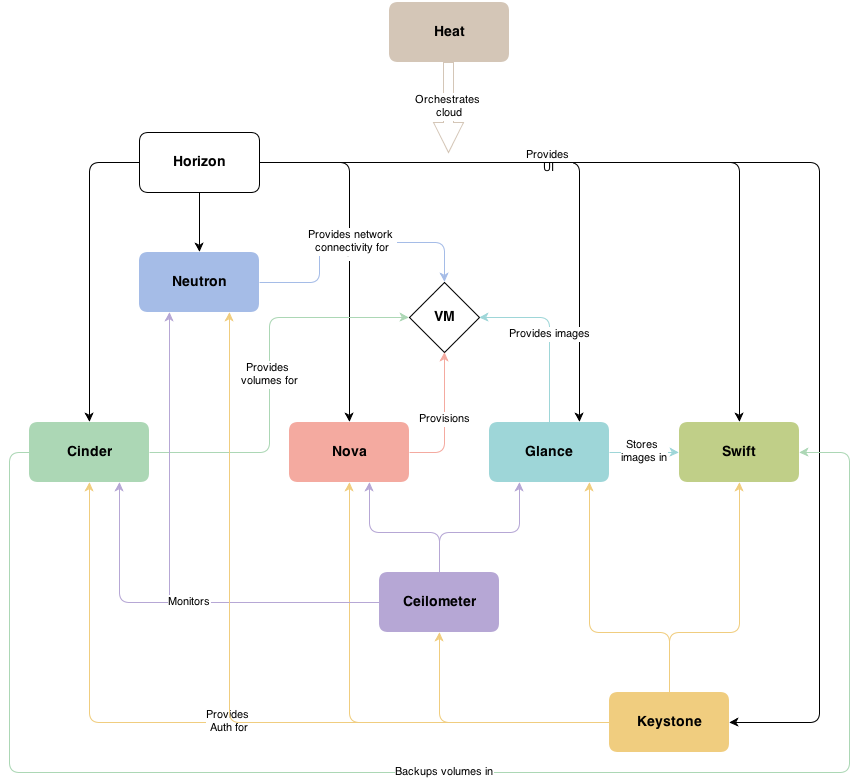
\includegraphics[scale=0.5]{figures/openstack_havana_conceptual_arch.png}
	\caption{Conceptual architecture of OpenStack Havana \cite{osarch}}
	\label{fig:openstack_services_arch}
\end{figure}

\begin{table}[h]
	\centering
	\begin{tabular}{|l|l|p{9.5cm}|}
		\hline
		\textbf{Project name} & \textbf{Service} & \textbf{Description}\\
		\hline
		Nova & Compute & Creates and manages virtual machines\\
		Keystone & Identity & Provides authentication and authorization\\
		Horizon & Dashboard & Web interface to manage all services\\
		Neutron & Networking & Manages networking for advanced network topologies\\
		Glance & Image & Provides a registry of virtual machine images\\
		Cinder & Block Storage & Provides persistent storage to VMs\\
		Swift & Object Storage & Stores data, including virtual images\\
		Ceilometer & Telemetry & Collects metering data (CPU and network costs)\\
		Heat & Orchestration & Deploys (complex) running cloud applications or stack (i.e. flavor, instance, network, etc.) described with templates (YAML text files)\\
		Trove & Database & Provides scalable and reliable cloud provisioning functionality for relational and non-relational database engines\\
		\hline
	\end{tabular}
	\caption{OpenStack services}
	\label{table:openstack_services_list}
\end{table}

\subsection{Nova}
Nova service is responsible for creating and managing virtual machines on demand.
Upon creating a virtual machine, the user can specify a flavor he wants to use.
The flavor allows to set the characteristics of a virtual machine: amount of RAM, number of virtual CPUs (VCPUs), sizes of root disk, ephemeral disk and swap disk. By default, Nova provides a set of flavors and the user can create more if needed.
Table \ref{table:flavors_list} shows characteristics for a list of the default flavors (ephemeral and swap disks are set to 0).

\begin{table}[h]
	\centering
	\begin{tabular}{|l|l|l|l|}
		\hline
		\textbf{Flavor} & \textbf{\# of VCPUs} & \textbf{Disk size (GB)} & \textbf{RAM size (MB)}\\
		\hline
		m1.tiny & 1 & 1 & 512 \\
		m1.small & 1 & 20 & 2048 \\
		m1.medium & 2 & 40 & 4096 \\
		m1.large & 4 & 80 & 8192 \\
		m1.xlarge & 8 & 160 & 16384 \\
		\hline
	\end{tabular}
	\caption{Flavors}
	\label{table:flavors_list}
\end{table}

OpenStack provides two different services to manage storage, namely \textit{Block Storage} and \textit{Object Storage}.
As mentioned earlier, the different OpenStack services can be installed separately, and one does not need to install all the services in order to have a virtual machine running.
\rp{you use phrases like ``said later''/``earlier'' way too often, try to reduce, I've already cut some.}
By default, when creating a virtual machine, it will have its own storage (i.e. a disk or a root disk), which is mandatory in order to install an operating system on it,
and it does not need the Block Storage service. 
The latter will be useful when one needs to extend the storage of a virtual machine in the future. 
Coming back to flavors, ephemeral disk corresponds to the amount of disk space to use for the ephemeral partition when a virtual machine is launched. 
These type of disks are bonded to the lifecycle of a virtual machine, meaning that if a virtual machine is terminated, all the data on the disk are lost. 
However, the data persist after rebooting a virtual machine. 
The root disk is a special case of ephemeral disk. 
It is used to create a root partition (/) for a virtual machine and, unlike ephemeral disk, it is included in snapshots of the virtual machine. 
If the size of the root disk is set to 0, this means that its size will be set to the one of image containing the operating system.
Finally, there is also the possibility to add a swap disk to the virtual machine.
The different storage solutions of OpenStack are summarized in Table \ref{table:storage_list}.

Nova is also able to handle networking thanks to the \texttt{nova-network} service. 
In this case, we talk about \textit{Legacy Networking} rather than \textit{OpenStack Networking} which refers to the Neutron project of OpenStack. 
As networking is very complex, it has been decided to split the Nova project in two parts: one project, Nova, will be exclusively responsible for virtual machines and another project, Neutron, will be exclusively responsible for networking. 
For our experiment, it was sufficient to only use Nova to manage networking instead of Neutron.


\begin{table}[h]
	\centering
	\begin{tabular}{|m{2cm}|m{3.8cm}|m{3.8cm}|m{3.8cm}|}
		\hline
		 & 
		\textbf{Ephemeral \newline storage} & 
		\textbf{Block storage} & 
		\textbf{Object storage}\\
		\hline
		\textbf{Used to} & 
		Run operating system and scratch space & 
		Add additional persistent storage to a virtual machine (VM) & 
		Store data, including VM images \\
		\hline
		\textbf{Accessed through} & 
		A file system & 
		A block device that can be partitioned, formatted, and mounted (such as, /dev/vdc) & 
		The REST API \\
		\hline
		\textbf{Accessible from} & 
		Within a VM & 
		Within a VM & 
		Anywhere \\
		\hline
		\textbf{Managed by} & 
		OpenStack Compute (nova) & 
		OpenStack Block Storage (cinder) & 
		OpenStack Object Storage (swift) \\
		\hline
		\textbf{Persists until} & 
		VM is terminated & 
		Deleted by user & 
		Deleted by user \\
		\hline
		\textbf{Sizing determined by} & 
		Administrator configuration of size settings, known as flavors & 
		User specification in initial request & 
		Amount of available physical storage \\
		\hline
		\textbf{Example of typical usage} & 
		10 GB first disk, 30 GB second disk & 
		1 TB disk & 
		10s of TBs of dataset storage \\
		\hline
	\end{tabular}
	\caption{Storage \cite{stodec}}
	\label{table:storage_list}
\end{table}


\subsection{Glance}
Glance is responsible for providing a registry of virtual machine images. 
The user is then able to easily retrieve an actual image for his virtual machine. 
An image contains an operating system image, which will be used to launch a virtual machine. 
The uploaded images are stored on the same system that hosts the Image Service, in the directory \texttt{/var/lib/glance/images/} by default.

\subsection{Cinder}
Cinder is responsible for providing persistent storage to virtual machines. 
The persistent storage is also called volume. 
Unlike ephemeral storage that was discussed before, all data that are on a volume persist when a virtual machine is terminated. 
This volume is similar to the Amazon Elastic Block Storage (EBS) 
and can be compared to an external hard disk drive (HDD) that is plugged into a computer: we say that the volume is attached to an instance. 
In order for the attached volume to be usable, it has to be mounted and formatted. 
After these steps, files can be stored on the volume. 
The attached volume can also be bootable, and thus replace the root disk seen before.
It has to be noted that one volume can only be attached to one instance at a time, but one instance can have several volumes attached to it.


\subsection{Keystone}
Keystone is responsible for providing authentication and authorization for the other OpenStack services and users. 
Therefore, it offers \textit{User management} and \textit{Service management}. 

The \textit{User management} lets one create users and tenants (or projects), the latter representing a group of users. 
The users will be able to connect to OpenStack by giving their credentials.
It is easy to have an overview of all running instances for the current tenant.
Also, it is possible to give specific roles to the users in a given tenant, so it's easy to restrict a user to only create instances for example. 

In order to manage services, the administrator has to first create a user per service. 
The \textit{Service management} provides identity, token, catalog and policy services.


% \begin{figure}[h]
% 	\centering
% 	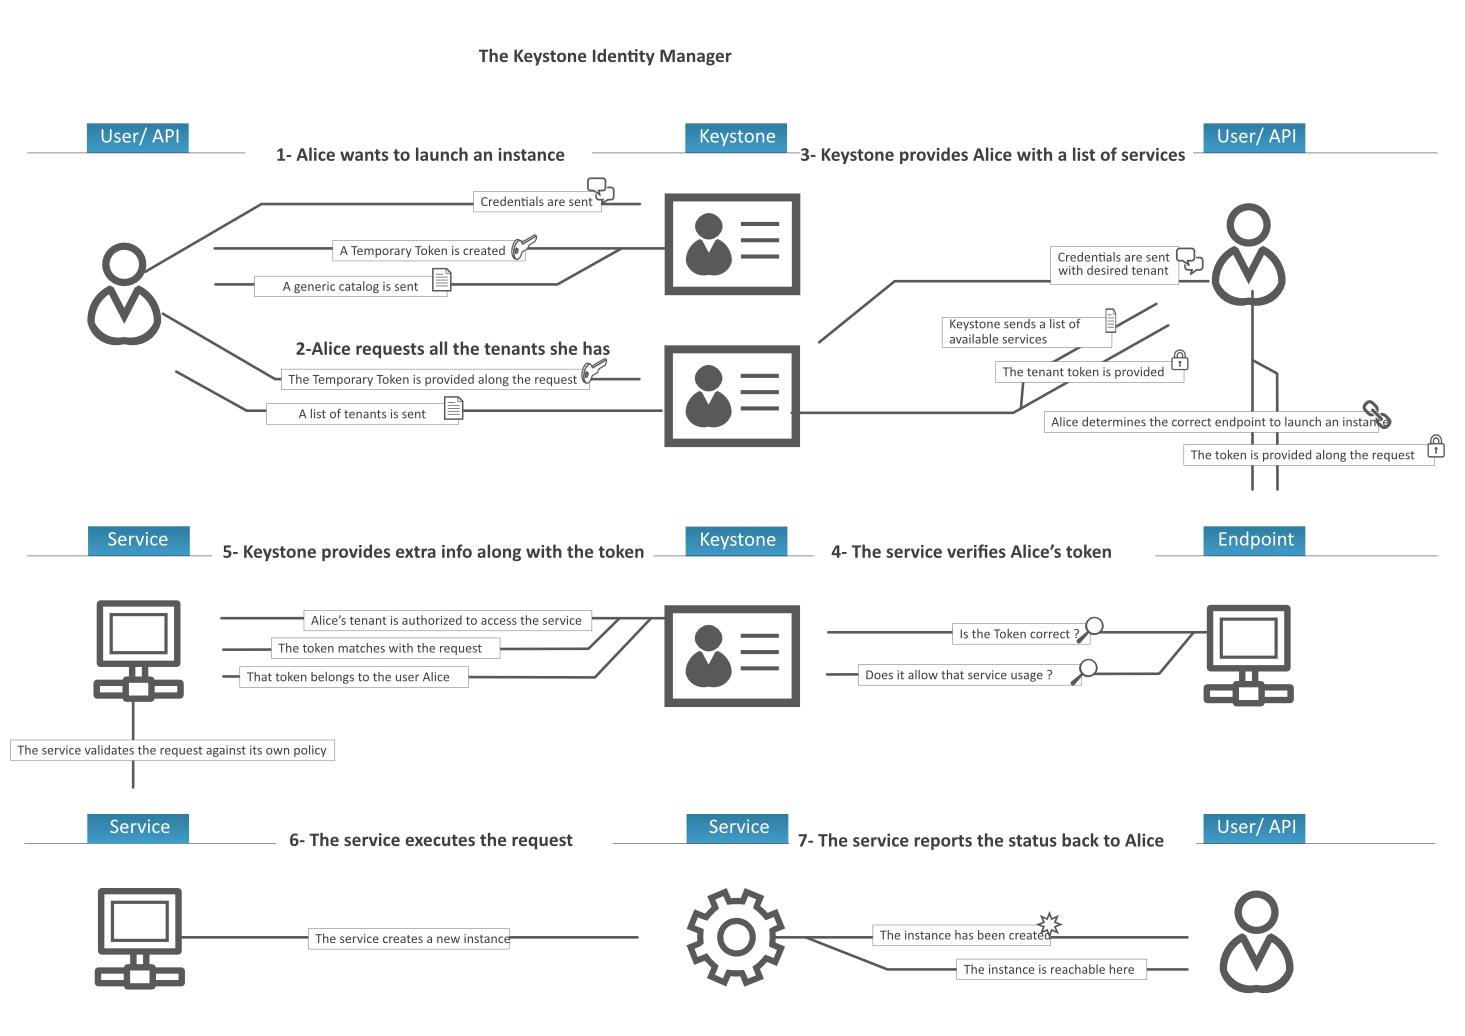
\includegraphics[scale=0.65, angle=90]{figures/keystone.png}
% 	\caption{Identity Service process flow}
% 	\label{fig:openstack_keystone}
% \end{figure} %%% [ref] http://docs.openstack.org/icehouse/install-guide/install/apt/content/keystone-concepts.html

\paragraph{Horizon}\mbox{}\\
Horizon provides a nice web interface (an example is shown in Figure \ref{fig:dashboard}) that lets users and administrators interact with OpenStack services easily, instead of executing commands through a terminal. 
However, Horizon cannot totally replace the command line tool.
Once logged in, users can launch instances and use it directly from a web browser thanks to VNC (or Virtual Network Computing) configured during the installation of OpenStack.








%%--------------- section
\section{Setup}
\label{section_setup}
For our experiments, OpenStack Icehouse was installed and configured on three physical machines:

{
\singlespacing
\begin{itemize}
	\item{\texttt{controller} which acts as a controller node}
	\item{\texttt{compute1} which acts as a compute node}
	\item{\texttt{compute2} which acts as a compute node and a block storage node}
\end{itemize}
}

As installing OpenStack is a relatively long process, all the steps won't be describe in this section. The OpenStack documentation \cite{osinstall}
descibes a well step-by-step that was followed in order to make everything work correctly.


\paragraph{Naming convention}\mbox{}\\
Virtual machines created on \texttt{compute1} will be called \texttt{vm1}, and those created on \texttt{compute2} will be called \texttt{vm2}. Moreover if the virtual machine has a block storage attached to it, \texttt{bs} will be attached to its name, becoming \texttt{vm1bs} for example. This convention will be followed for the rest of this report.


%%--------------- subsubsection
\subsection{Machines}
In this section, the hardware used for the experiments will be presented. We have three physical machines on which OpenStack services are installed, and several virtual machines with different flavors will be created on the physical machines with OpenStack.


\paragraph{Physical machines}\mbox{}\\
The three physical machines briefly presented in Section \ref{section_setup} are HP Compaq Elite 8300 SFF with a 64-bit architecture. 
Each machine uses a 3.4 GHz Intel Core i7-3770. 
There is 16GB of RAM, $4\times4$GB DIMM DDR3 Synchronous 1600MHz. 
They have a Western Digital HDD of 500GB. 
In the case of \texttt{compute2}, a partition of 100GB (93GB after partioning with GParted) has been created in order to have space for the Block Storage service of OpenStack instead of a full disk recommended by the OpenStack documentation. 
Physical and logical volumes have been created with LVM (Logical Volume Manager) for the partition created.
The machines are running Ubuntu 14.04 LTS 64 bit operating system. 
To create and run virtual machines, the open source hypervisor KVM (Kernel-based Virtual Machine) is used by the Compute Service. Concerning the network, each machine only have one interface card, instead of two interface cards recommended by the OpenStack documentation.



\paragraph{Virtual machines}\mbox{}\\
The virtual machines are created on \texttt{compute1} and \texttt{compute2} only and are using a cloud image\footnote{Ubuntu cloud images can be found here: \url{https://cloud-images.ubuntu.com}} of Ubuntu Server 14.04 LTS made to run on cloud platforms like OpenStack. 
A new flavor called \textit{physical} has been created and the flavor \textit{large} has been modified accordingly. 
The updated list of flavors is now represented on Table \ref{table:flavors_list_2}. 
For the experiments, only \textit{large} and \textit{physical} flavors are relevant. 
With the \textit{physical} flavor, we try to have similar characteristics as a physical machine in order to compare them. 
In this context, only one virtual machine with \textit{physical} flavor will be running at a time. 
With the \textit{large} flavor, we try to have half of characteristics of a physical machine in order to have enough resources to run two virtual machines at the same time to test isolation later.

\begin{table}[h]
	\centering
	\begin{tabular}{|l|l|l|l|}
		\hline
		\textbf{Flavor} & \textbf{VCPUs} & \textbf{Disk (in GB)} & \textbf{RAM (in MB)}\\
		\hline
		m1.tiny & 1 & 1 & 512 \\
		m1.small & 1 & 20 & 2048 \\
		m1.medium & 2 & 40 & 4096 \\
		m1.large & 4 & 30 & 8192 \\
		physical & 7 & 30 & 13312 \\
		\hline
	\end{tabular}
	\caption{Flavors}
	\label{table:flavors_list_2}
\end{table}



%%--------------- subsubsection
\subsection{OpenStack services} % TODO: or Components installation (?)
In this section, we will briefly explained which OpenStack services are installed on which physical machines and their purposes. The repartition of the different compoenents is shown in Figure \ref{fig:os_arch}.

\begin{figure}[h]
	\centering
	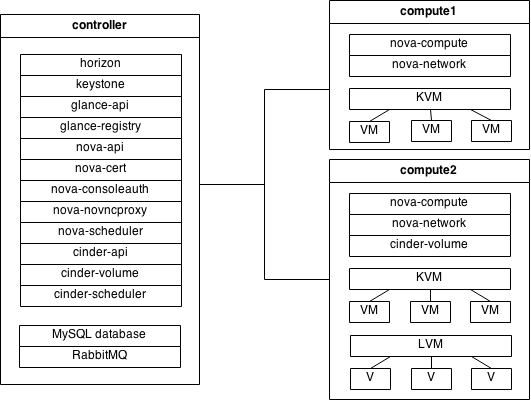
\includegraphics[scale=0.6]{figures/os_arch.png}
	\caption{Our OpenStack architecture}
	\label{fig:os_arch}
\end{figure}

First, let's take a look at \texttt{controller}. 
As its name suggests it, the controller node is the heart of our OpenStack architecture, and thus all the different services APIs (Application Programming Interface) are installed on it. 
Indeed, Keystone is there to manage users, and thus OpenStack services, as a user is created for each service. 
Each request made by a service is handled by Keystone first: the service must authenticate against Keystone, if this succeeds, then permissions are also checked, and if this is okay, the request is accepted and further actions can be done by the service who correctly authenticated itself. 
Glance (\textit{glance-api} and \textit{glance-registry}) is also installed on the controller node. 
This means that all actions regarding images (creation, edition, deletion) are handled by the controller node. 
Moreover all the different images are stored on it.
% TODO: put this text and the image in chapter 1 ?
A web interface makes OpenStack easier to use, and for that Horizon will be installed on the controller node, letting one access OpenStack with the following link \url{http://diufpc117.unifr.ch/horizon}\footnote{Access restricted to unifr network}. 
An overview of the dashboard is shown in Figure \ref{fig:dashboard}. 
As it can be seen, the dashboard offers access to each service installed, and as an administrator, it is possible to manage anything. 
To create, edit and delete an instance, a volume or an image, the user will access to these services through the \textit{Project} tab.
%
\begin{figure}[h]
	\centering
	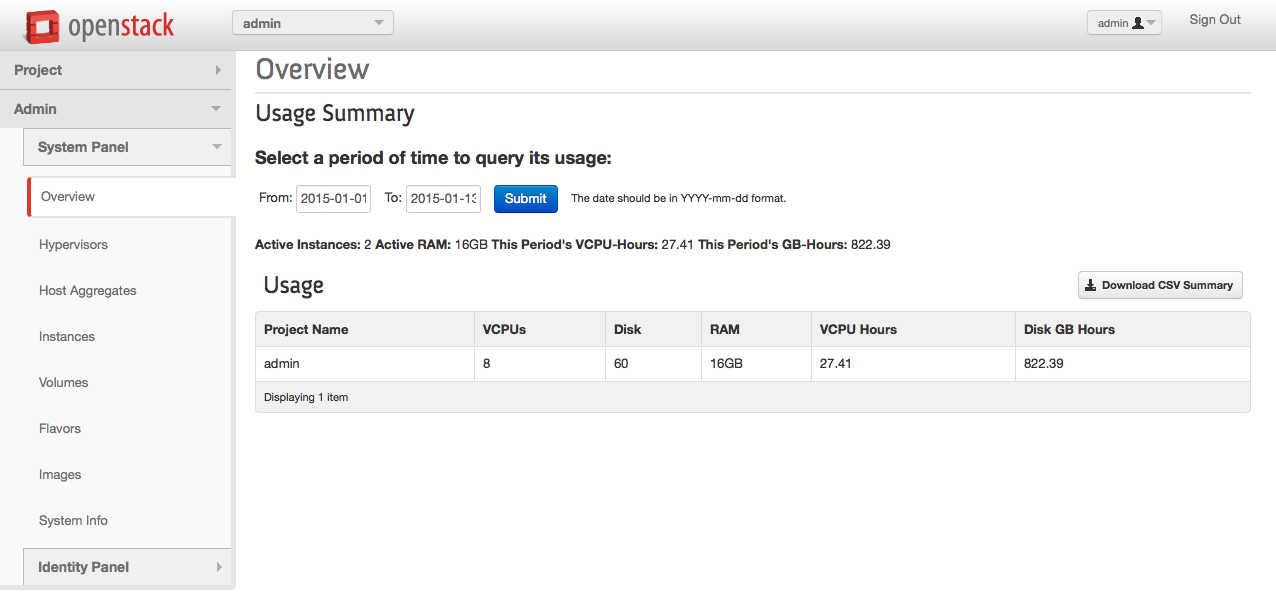
\includegraphics[scale=0.36]{figures/dashboard.png}
	\caption{Dashboard overview}
	\label{fig:dashboard}
\end{figure}
%
%TODO: nova -> describe each service?
In order to be able to create virtual machines, some components of Nova have to be installed on the controller node. These components are there for managing purpose. 
Among them, we can mention \textit{nova-api}, \textit{nova-cert}, \textit{nova-consoleauth} and \textit{nova-novncproxy} for accessing an instance via VNC, and \textit{nova-scheduler} to determine on which physical machine an instance will run.
Likewise, \textit{cinder-api}, \textit{cinder-volume} and \textit{cinder-scheduler} components of Cinder are installed on the controller for management purpose.
As each OpenStack needs to store some information, a database is necessary. 
For this a MySQL database is installed and configured on the controller node. 
On any additional node (in our case, on \texttt{compute1} and \texttt{compute2}), only a MySQL client is installed to access the database hosted on the controller node.
%TODO: messaging system?


Compared to the controller node, \texttt{compute1} and \texttt{compute2} are less complex and don't need to run as many services as the controller. 
For \texttt{compute1}, as its role is to create and host the virtual machines, other compoenents of the Nova project are needed: \textit{nova-compute}, which is responsible for creating and terminating virtual machines, and \textit{nova-network}, which is responsible for managing the network (bridging, updating iptables rules) for the virtual machines. 

Finally, \texttt{compute2} has the same compoenents as \texttt{compute1} regarding the Nova project. 
As this node also needs to take care of the creation and deletion of volumes, the \textit{cinder-volume} component of the Cinder project is present on the node. 





%%--------------- section
%!TEX root = ../main.tex
%% Chapter 3 - Benchmark


\chapter{Benchmark}
In computer science, a benchmark is an act of running a program that will put the machine under stress situation, in order to measure the performance. 
Several types of benchmarks exist in order to evaluate the performance of individual components of a machine. 
In the context of this bachelor work, a database benchmark has been run in order to evaluate the performance of OpenStack.
This section presents the tools and the benchmark used.

%%--------------- subsection
\section{TPC-C benchmark}
For our experiments, we used the TPC-C benchmark. 
TPC-C is defined as an \enquote{\textit{on-line transaction processing (OLTP) benchmark}}\footnote{\url{http://www.tpc.org/tpcc}, 14.09.2014} by the Transaction Processing Performance Council (TPC).
The performance of a given system is measured by simulating an OLTP database environment in which concurrent transactions happen.
Thus, a typical OLTP application depicting a wholesale supplier is used 
and only activities or tasks having an impact on resource utilization are considered, as they may affect the performance of the whole system.
This means that activities requiring small resource utilization and/or appearing with low frequency are completely ignored, 
letting just the most significant ones (Table \ref{table:tpcc_trans_type_list}) to evaluate the performance.
To better understand how this benchmark evaluates a system, one must understand how the chosen wholesale supplier is organized.
In this environment, we have a hierarchy. 
Beginning at the top, we have the company, which has several warehouses in different places, each one having 100000 items in stock.
Ten sales districts are distributed around each warehouse.
Each one of these sales districts serves 3000 clients (or customers).
The company receives new orders (composed of 5 up to 15 order lines) from clients.
The clients also have the possibility to check the statuses of their orders by contacting the company.
Among all the order lines, 1\% are for items that are not in-stock at a given warehouse.
These items have to be provided by another warehouse.
Finally, the company has to deal with clients' payments, order processing and stock levels.
Of course, as the business is growing, new warehouses and everything that comes after will be created.

\begin{table}[h]
	\centering
	\begin{tabular}{|m{4cm}|m{9cm}|}
		\hline
		\textbf{Transaction type} & \textbf{Description}\\
		\hline
		New Order & enters a new order into the database\\
		\hline
		Payment & updates the customer balance\\
		\hline
		Order Status & checks the status of an order\\
		\hline
		Delivery & processes batch of new orders not yet delivered\\
		\hline
		Stock Level & determines the number of sold items that have a low stock level (depending on threshold)\\
		\hline
	\end{tabular}
	\caption{TPC-C Transaction Types}
	\label{table:tpcc_trans_type_list}
\end{table}

From this system description, one can see that it has to deal with a lot of transactions, especially if the number of warehouses increases.
The corresponding TPC-C database, consisting of nine tables, is depicted by the entity-relationship diagram shown in Figure \ref{fig:tpcc_erd}.
One can see that the number of warehouses is the scale factor of this database, meaning that the more warehouses there are, the bigger the size of the database will be.
Indeed, the number of rows in each table is a function of the given number of warehouses.
The table ``Item'' is an exception and has a fixed number of rows.

\begin{figure}[h]
	\centering
	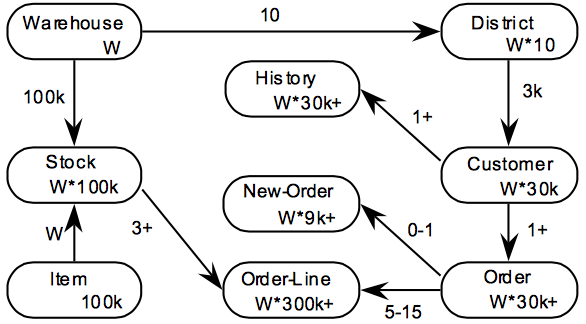
\includegraphics[scale=0.5]{figures/tpcc_erd.png}
	\caption{TPC-C database ER diagram \cite[p. 11]{tpcc10}}
	\label{fig:tpcc_erd}
\end{figure}

During a benchmark run, simulated users are interacting with the system by issuing different transactions, which are then processed by TPC-C.
It returns the performance in the number of transactions per minute C (tpmC, the letter \textit{C} denotes the type of benchmark which is TPC-\textit{C} in our case), which corresponds to the average number of new orders the system is processing per minute.
It is then straightforward to compare the performance of different systems.



%%--------------- subsection
\section{OLTP-Bench}
\textit{OLTP-Bench}\footnote{\url{https://github.com/oltpbenchmark/oltpbench}} is an open source project which aims to facilitate benchmarking by providing different ready to use benchmarks. 
Table \ref{table:oltpbench_list} summarizes the different benchmarks supported by this tool, which includes TPC-C benchmark presented in the previous section.
OLTP-Bench is a command line tool which is easy to use in order to populate a database and to run a benchmark.
Moreover, it allows to easily change parameters thanks to XML-based configuration files.
This configuration requires only few things like setting the connection to the database, the scale factor (which corresponds to the number of warehouses), the number of terminals (which corresponds to the number of simulated users, who will interact with the system (i.e. do business transactions)), the workload and the duration of the benchmark.
An example of such configuration is shown in Listing \ref{lst:lst_oltp_config}.
OLTP-Bench returns a throughput expressed in the number of requests per second (req/s), in contrast to tmpC in TPC-C specification.
This value is used to compare performances in different configurations.

OLTP-Bench is discussed in more details in Section \ref{sec:softwares} dedicated to the different software used for the experiments.

\begin{table}[h]
	\centering
	\begin{tabular}{|m{3.5cm}|m{3.5cm}|m{6cm}|}
		\hline
		\textbf{Class} & \textbf{Benchmark} & \textbf{Application domain}\\
		\hline
		\multirow{7}{*}{Transactional} & AuctionMark & On-line Auctions\\
		 & CH-benCHmark & Mixture of OLTP and OLAP\\
		 & SEATS & On-line Airline Ticketing\\
		 & SmallBank & Banking System\\
		 & TATP & Caller Location App\\
		 & TPC-C & Order Processing\\
		 & Voter & Talent Show Voting\\
		\hline
		\multirow{4}{*}{Web-Oriented} & Epinions & Social Networking\\
		 & LinkBench & Social Networking\\
		 & Twitter & Social Networking\\
		 & Wikipedia & On-line Encyclopedia\\
		\hline
		\multirow{4}{*}{Feature Testing} & ResourceStresser & Isolated Resource Stresser\\
		 & YCSB & Scalable Key-value Store\\
		 & JPAB & Object-Relational Mapping\\
		 & SIBench & Transactional Isolation\\
		\hline
	\end{tabular}
	\caption{Set of benchmarks supported in OLTP-Bench \cite{difallah14}}
	\label{table:oltpbench_list}
\end{table}




%%--------------- section
%% Chapter 4 - Experiments


\chapter{Experiments}
In this chapter, the practical part of this bachelor work will be presented.
First, a general decription of how the experiments is organized is presented.
Then, the choice of the different machines will be discussed in the Preliminary section.
For this choice, different little benchmarks have been used, which will be discussed.
Then, the configuration of the different physical and virtual machines will be presented in details, in order for these experiments to be reproductible.
The configuration includes the softwares installation and the tuning of MySQL.
Finally, the different tests and their results will be discussed.


%%--------------- section
\section{Description and procedure}
As already mentioned before in this document, a database benchmark, named TPC-C, has been chosen in order to evaluate the performance of OpenStack.
The OLTP-Bench project has been used to run TPC-C benchmark on the different physical and virtual machines running a MySQL server.
The virtual machines are created with different configurations (flavors, volume attached or not). 
It is expected to see the difference in performance for these different configurations and therefore the performance of OpenStack.
These results will be compared to the result obtained when running OLTP-Bench on the chosen physical machine (Section \ref{sec:preliminary} shows how this machine is choosen).

The tests are presented in four different phases.
In the first phase, OLTP-Bench is run on the physical machine chosen.
In the second, it is run on virtual machines with different flavors.
The third phase phase is similar to the second, except that a volume is attached to the virtual machine.
The last phase aims to test isolation, which is done by running OLTP-Bench on two different virtual machines at the same time.




%%---------------
%%--------------- section
%%---------------
\section{Preliminary}
\label{sec:preliminary}
Before beginning benchmarking with OLTP-Bench, we need to have a point of comparison, a machine with which we can compare all the results obtained. 
In order to choose this machine, the \texttt{hdparm} and Bandwidth benchmark have been used. 
These two little benchmarks will evaluate physical machine components (hard disk and memory).
Based on their results, a reference machine will be chosen and the experiments will begin.


\paragraph{HDPARM Benchmark}\mbox{}\\
%%--------------- begin: HDPARM
The \texttt{hdparm} is a command line program on Linuex systems and offers a bunch of parameters that lets one test the hardware of a machine in details. 
It should be noted that some parameters are risky and therefore has not been used for this experiment. 
Running the benchmark is pretty straightforward and is shown in Listing \ref{lst:lst_hdparm}.
In order to issue these commands, one must be root or use the command with \texttt{sudo}.

{
\singlespacing
\begin{lstlisting}[frame=single,language=bash,caption={hdparm commands},label={lst:lst_hdparm}]
#run on physical machines:
  $ hdparm -Tt /dev/sda1
#run on virtual machines:
  $ hdparm -Tt /dev/vda1
#run on virtual machines with a volume:
  $ hdparm -Tt /dev/vdb
\end{lstlisting}
}

The options \texttt{-Tt} allow to benchmark the reading speed of the hard disk drive (HDD) and the memory (RAM) without accessing the HDD. 
The returned values are an average speed expressed in MB/s. 
The value returned by the option \texttt{T} is \textit{Timing cached reads} and measures the reading speed of the RAM and swap in case the memory is full. 
The value returned by the option \texttt{t} is \textit{Timing buffered disk reads} and measures the reading speed of the HDD in the specified partition.
The commands were run six times and the average results are presented in Table \ref{table:hdparm_res_PM} for the physical machines. 

One can clearly see that \texttt{compute2} has the best performance regarding its hard drive, even if the difference with the two other machine is very small. 
Thus, this machine was chosen as a compute node and block storage node for OpenStack.
Thus, \texttt{compute2} is the reference machine with which benchmark results will be compared to.
The \texttt{compute1} machine was chosen as a compute node, as it has the highest value regarding the cached reads.
The \texttt{machine4} is not part of the experiments, even if it was a potential candidate from the results obtained in Table \ref{table:hdparm_res_PM}.

\begin{table}[h]
	\centering
	\begin{tabular}{|m{6cm}|m{2.5cm}|m{2.5cm}|m{2.5cm}|}
		\hline
		& 
		\texttt{compute1} & %vm116
		\texttt{compute2} & %vm115
		\texttt{machine4} \\
		\hline
		\textbf{Buffered disk reads (MB/s)} & 
		120.65 & 
		134.06 & 
		124.86 \\
		\hline
		\textbf{Cached reads (MB/s)} &  
		15428.67 & 
		15327.23 & 
		15408.54 \\
		\hline
	\end{tabular}
	\caption{hdparm results for physical machines}
	\label{table:hdparm_res_PM}
\end{table}

The same procedure is applied to virtual machines.
For this, virtual machines were created on the two machines selected before, \texttt{compute1} and \texttt{compute2}.
We expect to obtain similar results has the virtual machines are using the same hardware as their host.
The results are presented in Table \ref{table:hdparm_res_VM} for the virtual machines with flavors large and physical, and with and without a volume attached to it.

\begin{table}[h]
	\centering
	\begin{tabular}{|m{6.5cm}|m{1.5cm}|m{1.5cm}|m{1.5cm}|m{1.5cm}|}
		\hline
		\textbf{\textit{physical}} & 
		\texttt{vm1} & 
		\texttt{vm1bs} & 
		\texttt{vm2} & 
		\texttt{vm2bs} \\
		\hline
		\textbf{Buffered disk reads (MB/s)} & 
		126.61 & 
		110.8 & 
		117.58 & 
		320.44* \\
		\hline
		\textbf{Cached reads (MB/s)} &  
		14269.78 & 
		14223.5 & 
		15165.49 & 
		14890.86 \\
		\hline\hline
		\textbf{\textit{large}} & 
		\texttt{vm1} & 
		\texttt{vm1bs} & 
		\texttt{vm2} & 
		\texttt{vm2bs} \\
		\hline
		\textbf{Buffered disk reads (MB/s)} & 
		124.48 & 
		110.61 & 
		103.38 & 
		536.1* \\
		\hline
		\textbf{Cached reads (MB/s)} &  
		15520.6 & 
		15526.52 & 
		15372.97 & 
		15842.84 \\
		\hline
	\end{tabular}
	\caption{hdparm results for VMs}
	\label{table:hdparm_res_VM}
\end{table}

As one can observe, the results obtained with virtual machines are quite interesting.
Indeed, better results regarding hard disk are obtained for \texttt{vm1} hosted on the less performant machine \texttt{compute1}, and the opposite for \texttt{vm2}.
The fact is that this benchmark is run on a short period of time (2-3 seconds) and 
it's difficult to evaluate hard disk and memory performance as they are always used by the system (some running processes can affect the results). 
Other runs have shown lower performance results (around 105 MB/s) for \texttt{vm1} for example.
So, we can assume that both virtual machines (\texttt{vm1} and \texttt{vm2}) have quite similar performance and thus we expect to have quite similar results between them after running OLTP-Bench.
More interesting results are shown with values followed by a star (*). 
Indeed, they present quite high performance results when a volume (hosted on \texttt{compute2}) is attached to a virtual machine (also hosted on \texttt{compute2}).
When \texttt{hdparm} was run, the buffered disk reads result increased between each run and didn't stay stable like all other runs.
Thus, one can expect to observe a similar behaviour when running OLTP-Bench.
As a result, \texttt{vm2} is chosen as the reference machine (for the virtual machines), as it presents better performance results regarding the cached reads.
%%--------------- end: HDPARM


%%--------------- begin: RAM bandwidth
\paragraph{Bandwidth Benchmark}\mbox{}\\
In the same way as with \texttt{hdparm}, we also benchmarked the RAM with an open source program called \textit{Bandwidth}\footnote{\url{https://zsmith.co/bandwidth.html}, 14.09.2014}. 
This artificial benchmark was run in order to be sure that the RAM of each machine has the same performance, as we would have expected from the output of \texttt{hdparm} shown before.
As we were only interested in the first outputs of Bandwidth, we didn't run systematically the full test. Here is an excerpt of Sequentialial reads output from \texttt{vm2} with \textit{large} flavor:

\begingroup
	\singlespacing
    \fontsize{10pt}{12pt}\selectfont
\begin{verbatim}
    ...
    Sequential read (64-bit LODSQ), size = 128 B, loops = 241172480, 5879.4 MB/s
    Sequential read (64-bit LODSQ), size = 256 B, loops = 174587904, 8523.1 MB/s
    Sequential read (64-bit LODSQ), size = 384 B, loops = 134566740, 9848.3 MB/s
    Sequential read (64-bit LODSQ), size = 512 B, loops = 109969408, 10736.3 MB/s
    Sequential read (64-bit LODSQ), size = 640 B, loops = 94056729, 11474.7 MB/s
    Sequential read (64-bit LODSQ), size = 768 B, loops = 80740044, 11823.8 MB/s
    Sequential read (64-bit LODSQ), size = 896 B, loops = 71752284, 12255.5 MB/s
    Sequential read (64-bit LODSQ), size = 1024 B, loops = 64028672, 12500.3 MB/s
    Sequential read (64-bit LODSQ), size = 1280 B, loops = 52952280, 12920.0 MB/s
    ...
\end{verbatim}
\endgroup

Similar results are obtained for each physical and virtual machines. 
As it was expected, the performance doesn't change too much and tend to stay the same on each machine.
%%--------------- end: RAM bandwidth

\paragraph{OLTP-Bench configuration}\mbox{}\\
Now that we have our machine chosen, we can begin to run OLTP-Bench on it. 
Before running the tests, the database has to be filled up with the different scale factor: 1, 16, 32, 64, 74, 84, 94, 104. 
To do this we must first create the appropriate databases: tpcc\_1, tpcc\_16\_ tpcc\_32, tpcc\_64, tpcc\_74, tpcc\_84, tpcc\_94, tpcc\_104. 
Then we can issue the command in Listing \ref{lst:lst_cmd_oltpbenchmark} from the terminal to fill up the databases.

{
\singlespacing
\begin{lstlisting}[frame=single,language=bash,caption={oltp create},label={lst:lst_cmd_oltpbenchmark}]
  $ ./oltpbenchmark -b tpcc -c config/tpcc_s1_t40_config.xml \
    --create=true --load=true
\end{lstlisting}
}

Listing \ref{lst:lst_oltp_config} shows an example of a configuration file for OLTP-Bench. 
First we specify the connection details to access the database, then the scale factor and finally the workload. 
In the workload, only the number of terminals and the time the benchmark should last have been changed. 
Different configuration files were created in advanced in order to facilitate the execution of the different benchmarks. 
In order to do this, all configuration file name are following a convention, in which we specify the scale factor number (s1 in our example) and the number of terminals (t40 in our example).
With this, a little bash script \footnote{hosted on GitHub: \url{https://github.com/nad0u/oltpbench-run}, 20.05.2015}
has been created in order to launch one of the customed configuration file by specifying the scale factor as an argument (see example in Listing \ref{lst:lst_cmd_oltpsh}).
It is possible to enter more than one argument, in case one wants to launch several benchmarks with different scale factors.

{
\singlespacing
\begin{lstlisting}[frame=single,language=bash,caption={Bash script for launching benchmarks},label={lst:lst_cmd_oltpsh}]
  $ ./oltpbench-run 1
\end{lstlisting}
}

The command in Listing \ref{lst:lst_cmd_oltpsh} will look for the configuration file corresonding to the scale factor 1 (s1) and to 40 terminals (t40), and run the benchmark twice, saving all the data in folders which will be compressed.
The number of terminal must be changed in the script, same goes for the machine name on which the benchmark is run.
As a side note, this script will not create folder to store the results, they have to be created in advance and be named as \texttt{results\_sX} (X is the scale factor number).

{
\singlespacing
\lstset{
    language=xml,
    tabsize=3,
    %frame=lines,
    caption=OLTP-Bench configuration file example,
    label=lst:lst_oltp_config,
    frame=single,
    rulesepcolor=\color{gray},
    xleftmargin=20pt,
    framexleftmargin=15pt,
    keywordstyle=\color{blue}\bf,
    commentstyle=\color{gray},
    stringstyle=\color{red},
    numbers=left,
    numberstyle=\tiny,
    numbersep=5pt,
    breaklines=true,
    showstringspaces=false,
    emph={
    	parameters,
    	driver,
    	dbtype,
    	DBUrl,
    	username,
    	password,
    	isolation,
    	scalefactor,
    	terminals,
    	works,
    	work,
    	time,
    	rate,
    	weights,
    	transactiontypes,
    	transactiontype,
    	name
    	},
    emphstyle={\color{magenta}}
    }
    \lstinputlisting{"source_code/tpcc_s1_t40_config.xml"}
}







%%---------------
%%--------------- section
%%---------------
\section{Softwares}
\label{sec:softwares}
In this section, the actual softwares and their configuration used in order to run the benchmark will be presented.

As already explained, to run the benchmark we'll be using the OLTP-Bench project. 
We just need to clone the project from GitHub 
% (see Listing \ref{lst:lst_cmd_oltpb_cloning}) 
or download the project from GitHub if Git is not installed on the system. 
In order for OLTP-Bench to work, \textit{Ant} (version 1.9.3), \textit{Java} (version 1.7.0\_79) and \textit{MySQL} (version 5.5.43) need to be installed (see Listing \ref{lst:lst_cmd_others_install}). 
Once done, the OLTP-Bench system can be built with \textit{Ant}.


{
\singlespacing
\begin{lstlisting}[frame=single,language=bash,caption={Ant, Java and MySQL installation},label={lst:lst_cmd_others_install}]
  $ sudo apt-get install ant
  $ sudo apt-get install openjdk-7-jdk
  $ sudo apt-get install mysql-server
\end{lstlisting}
}

Instead of using the default configuration of MySQL, we'll be tuning server parameters with the help of a script, named \texttt{mysql\_start.sh} and provided on the wiki page of the OLTP-Bench project
\footnote{\url{http://oltpbenchmark.com/experiments/dbms_config/mysql_start.sh}}. 
This configuration is used for maximum performance. 
Before using the script, we need to create a new folder that will hold the database instead of the one used by default by MySQL. 
The database will be found in \texttt{/tmp/tpcc}. 
To prevent the \texttt{/tmp} folder to be cleaned after a reboot, we need to edit the file \texttt{/etc/default/rc5} and set \texttt{TMPTIME=-1}. 
Then we need to edit the \texttt{mysql\_start.sh} script accordingly by replacing the second line by \texttt{DATADIR=/tmp/tpcc}. 
Now we need to initialize the new MySQL data directory, shut down the current running MySQL service and start MySQL again with the script (see Listing \ref{lst:lst_cmd_mysql_start}).

{
\singlespacing
\begin{lstlisting}[frame=single,language=bash,caption={Ant, Java and MySQL installation},label={lst:lst_cmd_mysql_start}]
  $ sudo mysql_install_db --datadir=/tmp/tpcc --user=mysql
  $ sudo service mysql stop
  $ sudo ./mysql_start.sh
\end{lstlisting}
}

Once done, we are ready to start benchmarking, which will be described in the four following sections.







%%---------------
%%--------------- section
%%---------------
\section{Phase 1 - Physical machine}
In order to have a point of comparison, the OLTP-Bench programm will be executed on the physical machine that performs the best regarding \texttt{hdparm} results, namely \texttt{compute2}.
Before running the tests, we will fill up the database with the different scale factors: 1, 16, 32, 64, 74, 84, 94, 104 (see Listing \ref{lst:lst_cmd_oltpbenchmark}). 
The size of each filled database is shown in Table \ref{table:tab_oltpb_scalefactor}.

\begin{table}[h]
	\centering
	\begin{tabular}{*{9}{|c}|}
		\hline
		\textbf{Database} & 
		1 & 
		16 & 
		32 & 
		64 & 
		74 & 
		84 & 
		94 &
		104 \\
		\hline
		\textbf{Size (in MB)} & 
		93.6 & 
		1922.9 & 
		3134.5 & 
		5603.2 & 
		6628.3 & 
		7381.6 & 
		8285.6 &
		9121.8 \\
		\hline
	\end{tabular}
	\caption{Database sizes}
	\label{table:tab_oltpb_scalefactor}
\end{table}

Once the databases populated, we can run the benchmarks by using the \texttt{oltpbench-run} script. 
In order to maximize performance, all the OpenStack services will be shut down during the tests. 
Moreover, the machines will be rebooted after scale factor tests. 
It has to be noted that after each run, the database will grow as many writes occur. 
Despite this, the databases won't be refilled after each tests. 
Also, these tests were done with 40 terminals. 
The benchmark has been excuted two times, each run lasting 1800 seconds.

\begin{figure}[h]
	\centering
	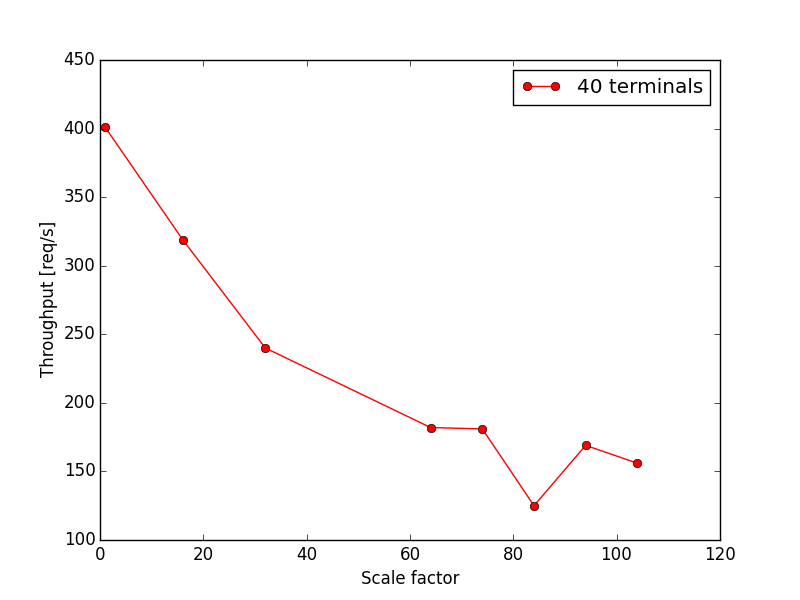
\includegraphics[scale=0.5]{figures/results/ph115_t40.png}
	\caption{\texttt{compute2} results}
	\label{fig:ph115_t40}
\end{figure}

As it can be seen in Figure \ref{fig:ph115_t40}, when the scale factor increases the throughput decreases. 
This behaviour is normal, as with a larger scale factor the database becomes bigger, and thus there is a lot more data to process and this will reduce the throughput of the system. 
For scale factor 84, we can see a little drop in the throughput. 
To be sure that this is just a "bad luck" during the benchmark, more runs can be done.

The throughput represented in the graph is computed by taking the 3600 throughput values ($2\times1800$ output values) of the OLTP-Bench output and calculating the first quartile $Q1$ and the third quartile $Q3$. 
The difference of $Q3$ and $Q1$ corresponds to the the interquartile range (IQR), which is a measure of statistical dispersion (see Equation \ref{eq:eq_iqr}). 
The final throughput will be computed by taking only output values between $Q1$ and $Q3$ included (or values in the IQR) and compute the median of these values.

\begin{equation}
   IQR = Q3 - Q1
   \label{eq:eq_iqr}
\end{equation}





%%---------------
%%--------------- section
%%---------------
\section{Phase 2 - Virtual machine without volume}
\label{section:phase2}

Like for the physical machine, databases will be created and populated before running OLTP-Bench. 
As the process of filling the databases is very long (especially with greater scale factors), snapshot of the virtual machine is taken.
All databases cannot be stored in only one virtual machine, which is made of a disk of 30 GB (as defined in Table \ref{table:flavors_list_2}).
So there will be two snapshots: one with databases with scale factors from 1 to 74, and the second one with the rest.
These snapshots are respectively named \textit{snap\_trusty\_16-74\_oltpsh\_} and \textit{snap\_trusty\_84-104\_oltpsh\_} on the web interface of OpenStack.
This way, it will be easy to destroy and create a new virtual machine with a different flavor and the populated database ready.

For this phase, OLTP-Bench was run on two different virtual machines with different flavors, \texttt{vm2} \textit{large} and \texttt{vm2} \textit{physical}. 
For the virtual machine with large flavor, OLTP-Bench was run with two different values for the terminals parameter: 1 and 40.
In the case of the physical flavor, OLTP-Bench was run only with 40 terminals.
Another thing to take care before running the benchmark on any \textit{large} flavored virtual machine: it is important to change the buffer pool size in the \texttt{mysql\_start} script. 
Otherwise, this will produce error as the buffer pool is as big as the RAM on the virtual machine.
The new value is set to 6G instead of 8G: \texttt{--innodb-buffer-pool-size=6G}.

\begin{figure}[h]
	\begin{minipage}{.5\textwidth}
		\centering
		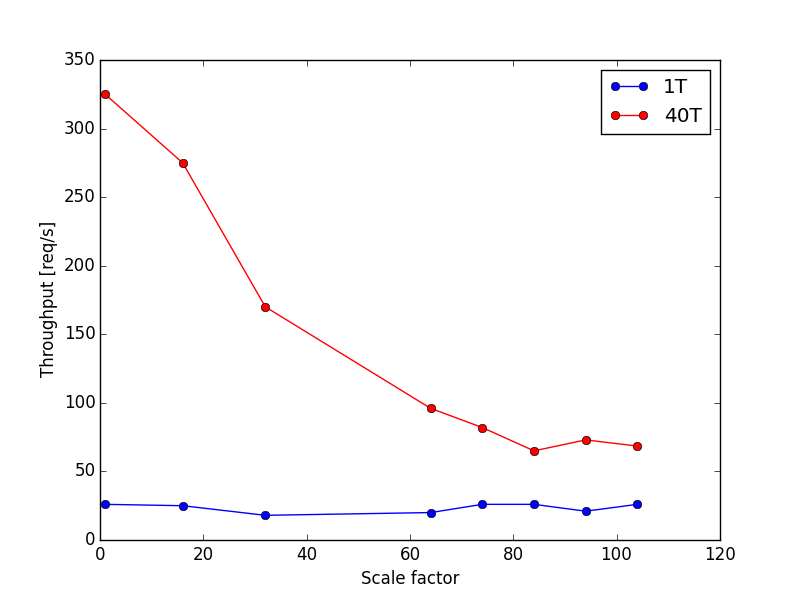
\includegraphics[scale=0.42]{figures/results/vm115_large_wobs.png}
		% \caption{\texttt{vm2} results for large flavor}
		\captionof{figure}{\texttt{vm2} results for large flavor}
		\label{fig:vm115_large_wobs}
	\end{minipage}
	\begin{minipage}{.5\textwidth}
		\centering
		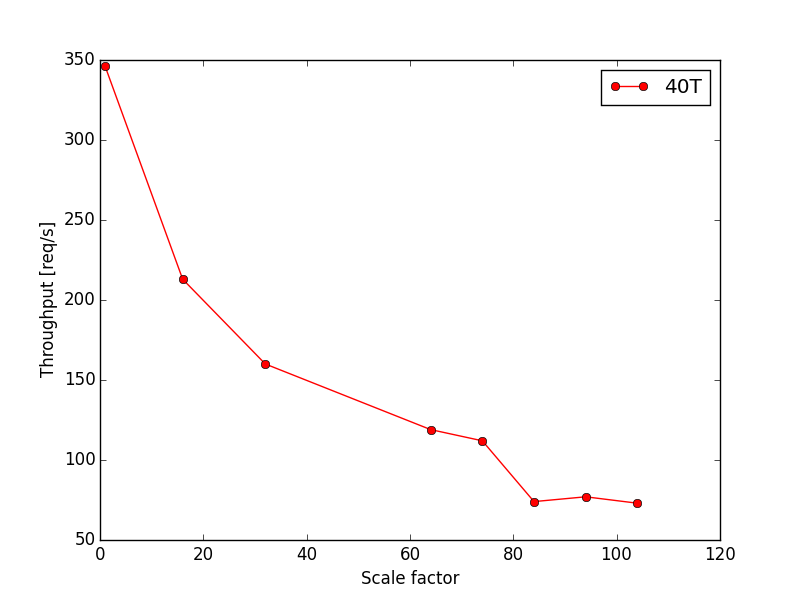
\includegraphics[scale=0.42]{figures/results/vm115_physical_wobs.png}
		% \caption{\texttt{vm2} results for physical flavor}
		\captionof{figure}{\texttt{vm2} results for physical flavor}
		\label{fig:vm115_physical_wobs}
	\end{minipage}
\end{figure}

As it can be seen in Figure \ref{fig:vm115_large_wobs} and \ref{fig:vm115_physical_wobs}, the throughput with 40 terminals are quite similar between the \textit{large} and \textit{physical} flavors. 
However, with scale factor 16, we observe a greater throughput loss with the \textit{physical} flavor compared to the \textit{large} flavor. 
Also, like with the results on \texttt{compute2}, we observe again a drop at scale factor 84, especially with the \textit{physical} flavor. 
It seems to be a coincidence, because an analysis of the data (plotting througput over time) shows that the benchmark crashes at some point (i.e. there is 0 values for quite some time).
This behavior appears quite frequently over all the different runs made, but in some case, like scale factor 84, this has a greater impact.
An example of such a crash is shown in Figure \ref{fig:vm115_physical_wobs_crash} (blue corresponds to the first run and red to the seconde run).
The crash begins after 450 seconds and lasts 150 seconds approximately.

\begin{figure}[h]
	\centering
	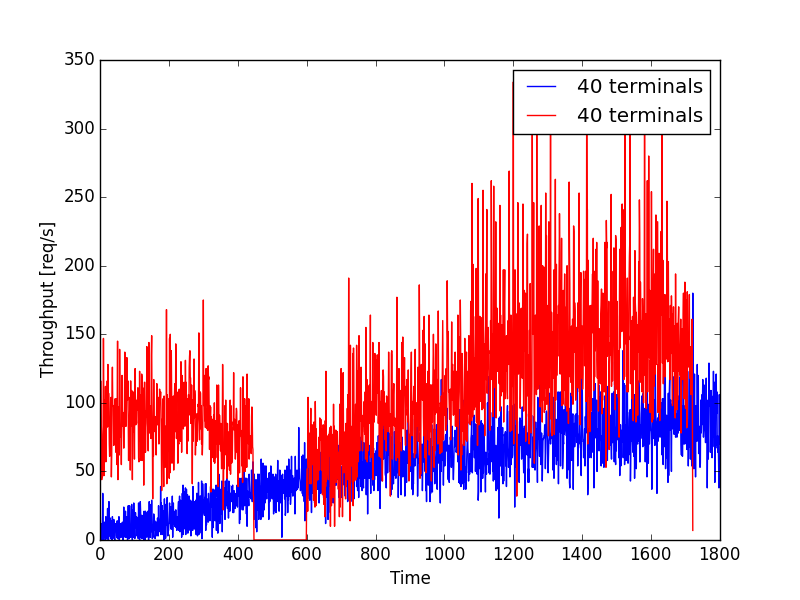
\includegraphics[scale=0.5]{figures/results/vm115_physical_wobs_crash.png}
	\caption{Crash on \texttt{vm2} physical (scale factor 84)}
	\label{fig:vm115_physical_wobs_crash}
\end{figure}

Concerning the results obtained with 1 terminal, we can see that they are quite constant.
It can be interesting to run the same benchmark with different values for the number of terminals in order to see where we have better performance.

Finally, one can observe that in general, better performances are achieved on \texttt{compute2} with a peak at 400 req/s for scale factor 1.
So, for now, OpenStack doesn't seems to beat performance of a physical machine, but it is quite close to.






%%---------------
%%--------------- section
%%---------------
\section{Phase 3 - Virtual machine with volume}

During this phase, the same tests as in Section \ref{section:phase2} will be run, but instead of using the ephemeral storage that comes with each virtual machine, we'll be using the OpenStack service for storage, known as Block Storage. The Block Storage service lets us create volume that can be seen as an external HDD that is attached to a computer. So basically, instead of storing the database in the default HDD of the virtual machine, it will be stored on the attached volume.

Before beginning the tests, some changes have to be made in order for everything to work. 
After changing the database location (moved on the attached volume), the AppArmor application will prevent MySQL to start, if it is not well configured. 
This application is installed by default on Ubuntu system, and is \textquote{\textit{a kernel-integrated application security system that controls how applications can access the file system}}
\footnote{\url{https://blogs.oracle.
com/jsmyth/entry/apparmor_and_mysql}, 17.02.2015}. 
As we are going to move the database on the attached volume, this new location must be known by the AppArmor application. 
Until now we didn't need to make any changes, as by default MySQL has access to the \texttt{/tmp} folder on Unix based system
\footnote{\url{http://dev.mysql.com/doc/refman/5.7/en/temporary-files.html}, 17.02.2015}. 
To attach a volume to the virtual machine, we need to create a new folder \texttt{/myspace} on which it will be mounted. 
The different commands to mount and move the database are shown in Listing \ref{lst:lst_cmd_mount_movedb}.

{
\singlespacing
\begin{lstlisting}[frame=single,language=bash,caption={Mount volume and move database},label={lst:lst_cmd_mount_movedb}]
  # Format the volume if it's not already done:
  $ mkfs -t ext4 /dev/vdb

  # Mount the volume on the created folder:
  $ mount /dev/vdb /myspace

  # Copy the databases and keep the same permissions:
  $ cp -rp /tmp/tpcc /myspace/
\end{lstlisting}
}

Once the data have been moved, we can shutdown MySQL and add the new database location to AppArmor (see Listing \ref{lst:lst_apparmor}). 
After reloading AppArmor, we also need to change the \texttt{DATADIR} variable in the \texttt{mysql\_start} script used for tunning MySQL. 
Instead of \texttt{DATADIR=/tmp/tpcc}, we have \texttt{DATADIR=/myspace/tpcc}. 
Now, we are ready to benchmark OpenStack using attached volumes to virtual machines.

{
\singlespacing
\begin{lstlisting}[frame=single,language=bash,caption={Configure AppArmor},label={lst:lst_apparmor}]
  # Add these two lines to /etc/apparmor.d/usr.sbin.mysqld
  /myspace/tpcc/ r,
  /myspace/tpcc/** rwk,

  # Reload AppArmor
  $ /etc/init.d/apparmor reload
\end{lstlisting}
}

For this part of the experiment, we wanted to see if the use of volumes attached to virtual machines can affect the performance, as it was observed when running \texttt{hdparm}. 
In particular, we want to see what happens when we have both the virtual machine and the volume hosted on the same physical machine (on \texttt{compute2} in our case) and when we have a virtual machine hosted on \texttt{compute1} and the volume hosted on \texttt{compute2}.

\begin{figure}[h]
	\begin{minipage}{.5\textwidth}
		\centering
		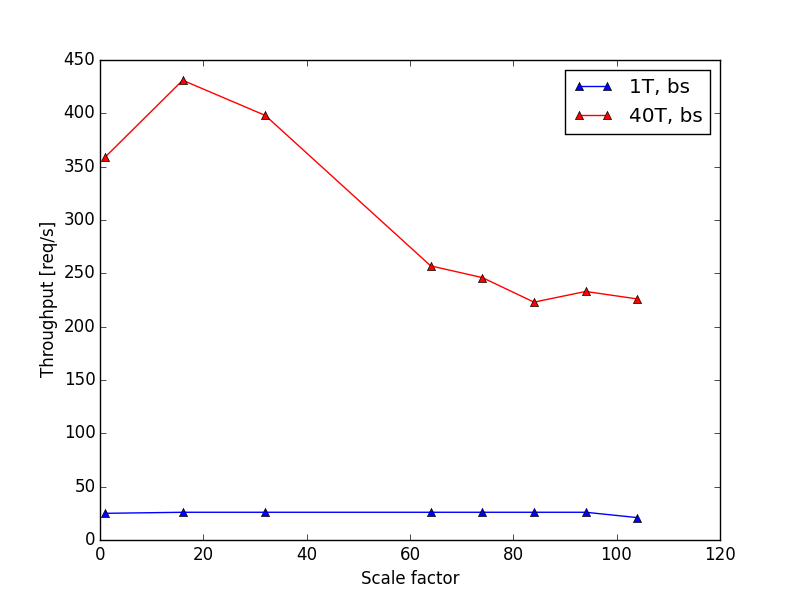
\includegraphics[scale=0.42]{figures/results/vm115_large_wbs.png}
		\captionof{figure}{\texttt{vm2bs} results for large flavor}
		\label{fig:vm115_large_wbs}
	\end{minipage}
	\begin{minipage}{.5\textwidth}
		\centering
		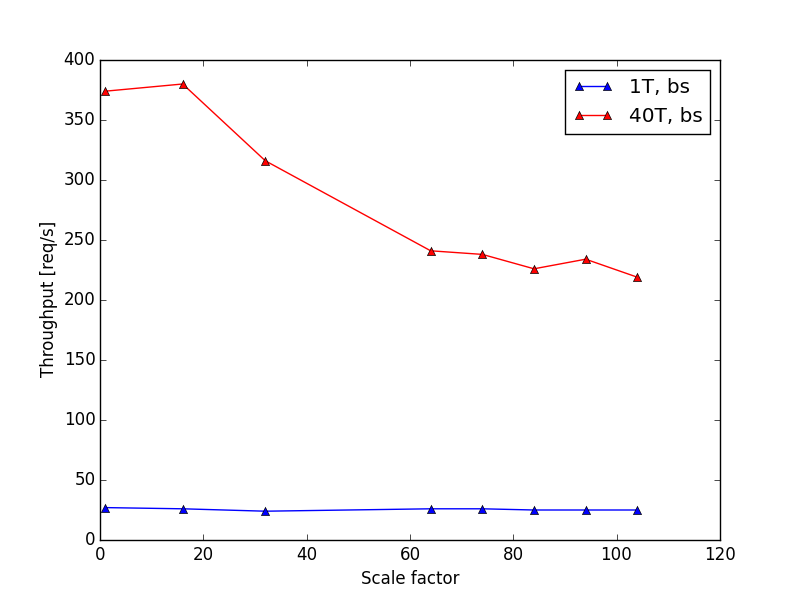
\includegraphics[scale=0.42]{figures/results/vm116_large_wbs.png}
		\captionof{figure}{\texttt{vm1bs} results for large flavor}
		\label{fig:vm116_large_wbs}
	\end{minipage}
\end{figure}

Like before, \textit{large} and \textit{physical} flavor will be used, and in the case of \textit{large} flavor, the benchmark will be run with 1 and 40 terminals. 
We will first discuss the case of \textit{large} flavor, whose results are shown in Figures \ref{fig:vm115_large_wbs} and \ref{fig:vm116_large_wbs}.
At first glance, we can see that both graphs have the same shape. However this shape differs from the results obtained in Phase 2. 
In the case of 40 terminals, we see that the throughput increases from scale factor 1 to 16, instead of decreasing like before. 
Moreover, in the case of scale factor 1, we can see that the throughput is at least around 350 req/s and goes up to around 430 req/s in the case \texttt{vm2bs}.
Thus, compared to \texttt{compute2}, we can reach a higher throughput.

For the other scale factors, one can observe that the throughput decreases like previous results in Phase 2, except that at the end (scale factor 104), the throughput stagnates at a higher level around 225 req/s instead of 75 req/s in results obtained in Phase 2. 
In fact, the throughput never goes below 200 req/s. 
Most of the results lie between 200 req/s and 260 req/s, which is clearly better than results obtained in Phase 2, and even better that the results obtained in Phase 1 where most of the results are below 200 req/s. 
Finally, as to be expected, the results for 1 terminal are constant and there is no higher throughput as there is only one client interacting with the database. 

Now, comparing \texttt{vm2bs} and \texttt{vm1bs} results, we see that we obtain slightly better performance results for \texttt{vm2bs}, especially for scale factors 16 and 32. 
So one can say that having an attached volume hosted on the same physical machine as the virtual machine potentially increases the performance in the case of \textit{large} flavor.

For the case of \textit{physical} flavor, one can observe a similar shape as we had in Figures \ref{fig:vm115_large_wbs} and \ref{fig:vm116_large_wbs}, except that the throuhput drops rapidly under 300 req/s for scale factore 32.
And as expected, the performance is way better than what was obtained in Phase 2 (see Figure \ref{fig:vm115_large_wobs}). 
Indeed, throughputs are always above 200.

\begin{figure}[h]
	\begin{minipage}{.5\textwidth}
		\centering
		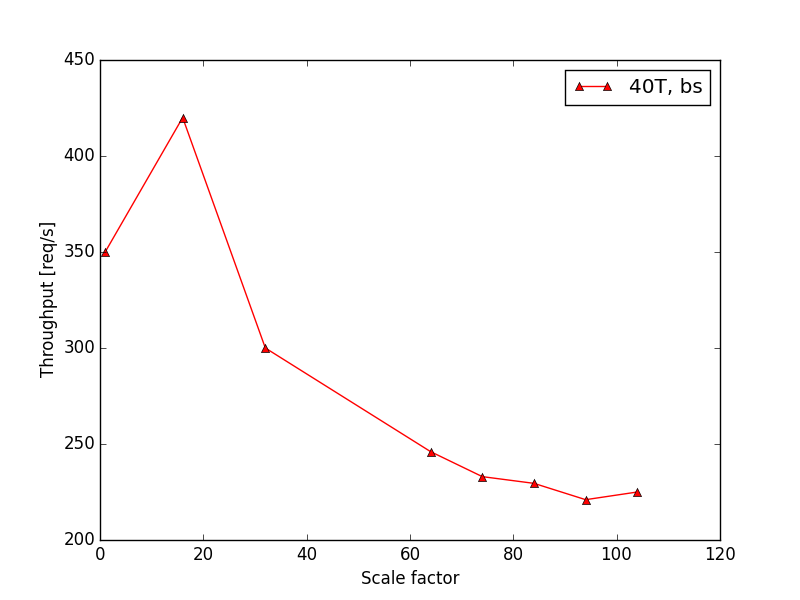
\includegraphics[scale=0.42]{figures/results/vm115_physical_wbs.png}
		\captionof{figure}{\texttt{vm2bs} results for physical flavor}
		\label{fig:vm115_physical_wbs}
	\end{minipage}
	\begin{minipage}{.5\textwidth}
		\centering
		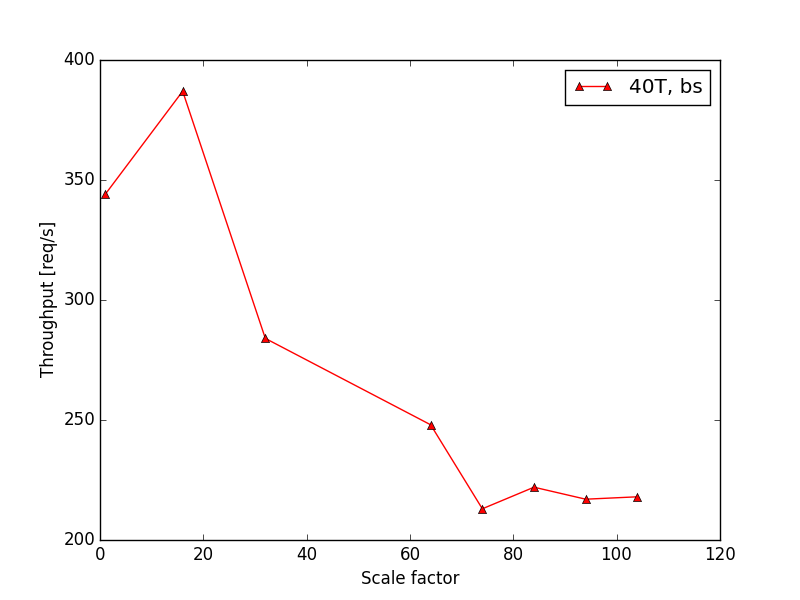
\includegraphics[scale=0.42]{figures/results/vm116_physical_wbs.png}
		\captionof{figure}{\texttt{vm1bs} results for physical flavor}
		\label{fig:vm116_physical_wbs}
	\end{minipage}
\end{figure}


Finally, as we can see, there is very little difference in performance between \textit{large} and \textit{physical} flavor when a volume is attached to the virtual machine. 
However, we obtain better performance compared to virtual machines without volume (see Figures \ref{fig:vm115_large_wobs} and \ref{fig:vm115_physical_wobs}). 
To conclude, we can say that having a volume attached to a virtual machine really improve the overall performance of the system.
Apparently, OpenStack is doing a great job with volumes managements.




%%---------------
%%--------------- section
%%---------------
\section{Phase 4 - Virtual machines isolation}

As a final step for this project, we wanted to test isolation between the virtual machines.
Indeed, when several virtual machines are hosted on the same physical machine, they have to share the available hardware components (i.e. CPU, HDD, RAM) of the host.
Testing isolation allows us to verify that a virtual machine is not interfering (or not interfering too much) with another virtual machine running on the same host. 
It must also be the case when two virtual machines are running on two different hosts. 
Thus, a good isolation allows to keep individual performance of each virtual machine more or less intact.
The isolation is particularily important in \textit{Cloud Computing} as each hardware resources can be rented on demand. 
Each customer that rented a virtual machine expects it to run at full power (the power he paid for), and so other virtual machines should not interfere with this rented one.

\begin{figure}[h]
	\centering
	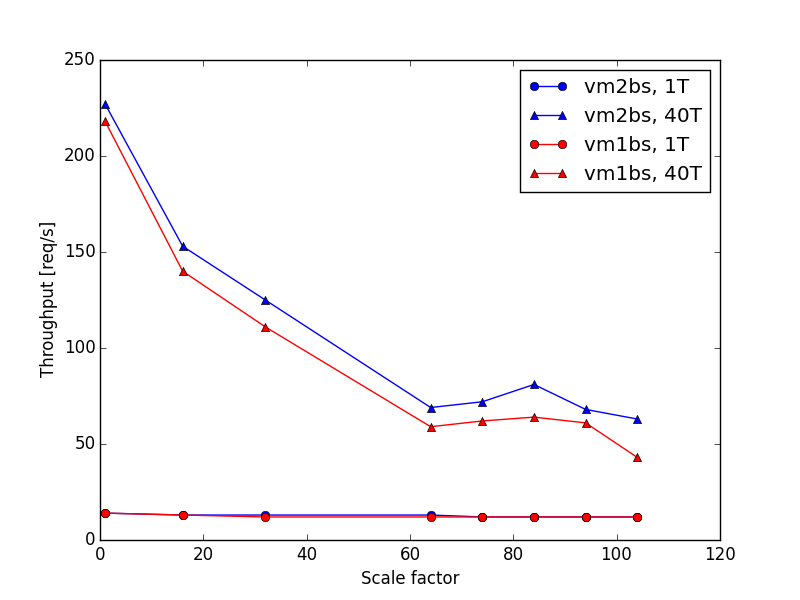
\includegraphics[scale=0.5]{figures/results/vm_large_iso.png}
	\caption{\texttt{vm1} (in red) and \texttt{vm2} (in blue) results for large flavor}
	\label{fig:vm_large_iso}
\end{figure}

In order to test isolation, we will consider the case where we have two virtual machines, \texttt{vm1} and \texttt{vm2}, running on two different physical machines, \texttt{compute1} and \texttt{compute2} respectively. 
Both virutal machines are created with \textit{large} flavor and have a volume attached to them. 
OLTP-Bench is executed at the same time on both virtual machines. 
As before we are considering two different number of terminals, 1 and 40. 
The results of the experiments are shown in Figure \ref{fig:vm_large_iso}.

Unfortunately, this test doesn't return good results.
Indeed, almost all throughput lie below 200 req/s, which is clearly worse than all results obtained until now.
This can be explained by the fact that we don't have a dedicated machine for managing the volume, a Block Storage node, in our OpenStack architecture.
This means that the two virtual machines try to access the same physical hard drive (where the database resides) during the benchmark, even if there is two logical volumes.

In order to better test isolation, one must consider having a dedicating machine for managing volume instead.
One can also try to run the same benchmark, without using volumes.
But as Phase 3 shown that better performance can be achieved by attaching volumes to the virtual machines, it seems logical to test isolation with volume also.





%%--------------- section
%!TEX root = ../main.tex
%% Conclusion


\chapter{Conclusion}
In this chapter summarizes the findings of this bachelor work, discusses the encountered problems and outlines potential future work.


%%--------------- section
\section{Findings}
The goal of this bachelor work was to get to know OpenStack, an open source cloud infrastructure project, and benchmark it.
As a personal note, no knowledge in the field of \textit{Cloud Computing} was there beforehand, especially in how everything works in details.
The only knowledge was those of an end-user just using data storage services like Dropbox, and being happy that it works well.
This bachelor work was a great opportunity to deepen these knowledge, by getting to know how everything works behind the scene, or how to setup a cloud infrastructure and being able to use it.

Coming back to the main topic, in order to be able to benchmark OpenStack, virtual machines created with OpenStack were benchmarked with the help of the OLTP-Bench project, an open source project supporting several types of benchmarks including TPC-C.
The benchmark was first run on a dedicated physical machine, whose results are used for comparison with the other benchmarks.
In order to benchmark OpenStack, the OLTP-Bench was run on virtual machines with different flavors and with or without logical storage attached to them.
In Phase 2 (virtual machines without storage), we obtained quite good performance results, but OpenStack could not outperform the the physical machine from Phase 1.
In Phase 3 (virtual machines with storage), we obtained very good results, even better than the physical machine.
From this we can conclude that attaching volumes to virtual machines can really improve the performance, and that OpenStack manages well the volumes.
In Phase 4 (testing isolation), the results obtained are not quite good, this is caused by the fact that both virtual machines are accessing the same hard drive hosted on \texttt{compute2}.

From these three phases, we can conclude that OpenStack is quite performant and can even perform better than physical machines.
Also, we observed that in general there is little difference in performance when comparing \textit{large} and \textit{physical} flavor virtual machines.
To be sure of this fact, it could be interesting to run the same benchmark on a virtual machine with \textit{small} or \textit{tiny} flavors.
A general observation, is that when the scale factor increases, the throughput of the system decreases.

Finally, OpenStack is a very interesting open source project that is gaining in popularity as a free IaaS.
Its performance is quite good, which is important in \textit{Cloud Computing} as its goal is to deliver computational power on demand.
The web interface is very intuitive and facilitates the management of the cloud infrastructure after a successful setup.







%%--------------- section
\section{Problems}
During this bachelor work, several problems arose at different stages. 
At first, we encountered problems when installing OpenStack on the different physical machines.
The process is very long as there is no ``one click'' setup as one could expect with a simple software installation.
OpenStack relies on configuration files after installing the different components.
This is where problems arose, as sometimes there were some little errors in the official documentation.
For example, it was specified that only the hostname of a machine can be used instead of giving the IP address for certain configuration files; but in reality, it was necessary to use the IP address instead. 
This type of error is quite minor (it was encountered when setting up VNC) and is easily solved if the status of OpenStack is checked at each step of the installation.
We also encountered network problems during the installation: at some point, it was possible to create instances but there were no IP assigned to them, and thus it was impossible to SSH the virtual machines.
This was solved by reserving IP addresses from the university network.

Concerning the benchmarks, it took a few attempts in order to find a good configuration to run the tests.
At first we only tried the default values\footnote{\url{https://github.com/oltpbenchmark/oltpbench/blob/master/config/sample_tpcc_config.xml}, 21.05.2015}, and observed that after each run the throughput was increasing.
So we did not know how many runs it was necessary to perform in order to have meaningful data.
We tried several configurations by increasing the duration and the scale factor.
We finally decided to use the values presented in the Listing \ref{lst:lst_oltp_config}.


%%--------------- section
\section{Future work}
With the different tests performed, we obtained quite useful insights regarding the OpenStack performance.
Below there are some other suggestions that could be used to obtain more meaningful results.

First, as it has been shown in Phase 4, it could be more interesting to use a machine dedicated to volume management in order to test isolation.
Better performance results might be observed.
One can also try to run the same benchmark as in Phase 4, without using volumes.
But as Phase 3 shown that better performance can be achieved by attaching volumes to the virtual machines, it seems logical to test isolation with volume also.

Then, other tests (for all Phases) can be performed by increasing the duration of a run. 
It could be better to extend the duration to 40 minutes for example.
Also, different number of terminals (20 and 80) can be used to see their impact on the performance.















%%--------------- section
%\chapter*{References}
\begin{thebibliography}{9}

%%%%%%%%% ---------- Literature source
\bibitem{osinstall}
	OpenStack, \emph{OpenStack Installation Guide for Ubuntu 12.04/14.04 (LTS)}. 
	Online guide, 
	\url{http://docs.openstack.org/icehouse/install-guide/install/apt/content/}, 
	2014.

\bibitem{osconfref}
	OpenStack Foundation, \emph{OpenStack Configuration Reference}, 
	\url{http://docs.openstack.org/icehouse/config-reference/content/}, 
	2014.

\bibitem{osopsguide}
	OpenStack Foundation, \emph{OpenStack Operations Guide}. 
	Online book,
	\url{http://docs.openstack.org/openstack-ops/content/}, 
	2014.

\bibitem{osimgguide}
	OpenStack Foundation, \emph{OpenStack Virtual Machine Image Guide}. 
	Online guide,
	\url{http://docs.openstack.org/image-guide/content/}, 
	2014.

\bibitem{difallah14}
  Djellel E. Difallah and Pavlo, Andrew and Curino, Carlo and Philippe Cudr{\'e}-Mauroux,
  \emph{OLTP-Bench: An Extensible Testbed for Benchmarking Relational Databases}.
  Online article, \url{http://exascale.info/sites/default/files/p260-difallah.pdf}, 
  2014.

 \bibitem{tpcc10}
  Transaction Processing Performance Council (TPC),
  \emph{TPC BENCHMARK\textsuperscript{TM}C, Standard Specification}.
  Online article, \url{http://www.tpc.org/tpc_documents_current_versions/pdf/tpc-c_v5-11.pdf}, 
  2010.


% %%%%%%%%% ---------- Citation source
\bibitem{cjanssen14}
	Cory Janssen,
	\emph{IT Infrastructure}, 
	\url{http://www.techopedia.com/definition/29199/it-infrastructure}, 
	Last visited: 15.09.2014.

% \bibitem{osdef}
% 	OpenStack: The Open Source Cloud Operating System, 
% 	\url{http://www.openstack.org/software/}, 
% 	Last visited: 15.09.2014.

% \bibitem{stodec}
% 	Storage Decisions, 
% 	\url{http://docs.openstack.org/openstack-ops/content/storage_decision.html}, 
% 	Last visited: 15.09.2014.



% %%%%%%%%% ---------- Figures source
% \bibitem{osarch}
% 	Architecture, 
% 	\url{http://docs.openstack.org/icehouse/install-guide/install/apt/content/ch_overview.html}, 
% 	Last visited: 15.09.2014.


\end{thebibliography}
% \bibliographystyle{plain}
% \bibliography{biblio}








%%--------------- section
% \chapter*{Glossary}









%%--------------- section
% \chapter*{Annexes}




\end{document}  